\documentclass[a4paper,12pt,titlepage]{article} % [papersize,fontsize,add title page]{document type}

% This LaTeX file can be turned straight into a pdf by "PDFTeXify" in WinEdit, or
% by any LaTeX --> PDF command in another LaTeX editor
%
% Because figure files are PDF, LaTeX --> DVI does not work

% usepackage{.} reads in additional LaTeX packages
\usepackage[pdftex]{graphicx}       % to include graphs
\usepackage{natbib}                % A BibTeX style file for references.
\usepackage{amssymb,amsmath}        % for maths symbols and equation numbering
\usepackage{array,tabularx,calc}
\usepackage{multirow} % create the tables
\usepackage{lscape} %put table lscape
\usepackage{pdflscape} %put pages lscape
\usepackage{listings}
\usepackage[T1]{fontenc}   %for the ""
\usepackage[title]{appendix} %for appendix

\newenvironment{conditions}[1][where:]
{%
	#1\tabularx{\textwidth-\widthof{#1}}[t]{
		>{$}l<{$} @{${}={}$} X@{}
	}%
}
{\endtabularx\\[\belowdisplayskip]}

% set up title page
\title{The NIR Corn Data Set}
\author{Hongwei PENG \vspace{2cm} \\
	Supervisor : Prof Tom Fearn \vspace{2cm} \\
	Department of Statistical Science \\
	University College London}
\date{\today} % \today gives today's date. ... or put in the date you want

% set page size and margins
\setlength{\textwidth}{17cm}
\setlength{\textheight}{26cm}
\setlength{\oddsidemargin}{-0.5cm}
\setlength{\evensidemargin}{-0.5cm}
\setlength{\topmargin}{-25mm}
\setlength{\parindent}{0cm}
\setlength{\parskip}{0.3cm}

\let\leq=\leqslant   % for nice-looking inequality signs
\let\geq=\geqslant

\numberwithin{equation}{section}  % equation numbers like (section#.equation#)

\linespread{1}     % 1: single-spacing, 2: double-spacing, 1.5: 1.5-spacing etc

\begin{document}   % start of document
	\maketitle         % create title etc
	
	\section{Abstruct} 
	These algorithms will often claim that their new algorithm has a better performs. So the purpose of this dissertation is to search for as many different papers as possible, and write a critical overall to find the most efficient measure that can evaluate whether the model performs well and quantify the improvements mentioned in the paper.
	\newpage           % start a new page
	
	\section{Acknowledgements} 
 	I would thank
	\newpage           % start a new page
	
	\tableofcontents   % create table of contents
	\newpage           % start a new page
	

	
	\section{Introduction}             % start a new section called `Introduction'
	\label{sec:intro}                  % create label for this section
	
	Introduction
	The near-infrared spectroscopy mainly reflects the frequency of the vibration of the hydrogen-containing group and the absorption of the frequency doubling at each level. Infrared spectroscopy combined with chemometric methods have been widely used for the detection of various plant samples. When the samples of plants are tested by near-infrared spectroscopy, this method is cheaper and faster than the traditional chemical method.
	
	However, although the spectroscopy technique is more convenient, for some samples with similar properties, it is impossible to draw an identification conclusion through an intuitive method. Because the detected high-dimensional data can not be read directly. Therefore, a stoichiometric method is needed to establish a prediction model in which spectral information is associated with sample features. Because spectral information belongs to high latitude data and has strong collinearity, choosing the appropriate regression method is very important for predictive models. Among them, common spectral data modeling methods include partial least squares and principal component regression. Among them, partial minimization multiplication has many applications in spectral analysis, and it is a very effective chemometric method. The partial least squares method can not only comprehensively screen out significant spectral data but also eliminate spectral collinearity problems. The main idea of the algorithm is to simplify the data structure and highlight the main contradictory multivariate statistical methods.
	
	The infrared spectral data of corn is the most easily obtained high-dimensional infrared spectrum data on the network. In recent years, many papers have analyzed corn data as an example. The most common algorithm for analyzing corn infrared spectral data is the partial least squares method. The partial least squares method can effectively reduce the dimensionality of the infrared spectrum. This is one of the best ways at the moment. Therefore, a large part of the paper is based on the partial least squares method to improve the accuracy of the prediction. And this type of paper also claims that its method has better performance than partial least squares. E.g:   
	
	Although this type of algorithm does show better performance from the results of the data, even if you choose the same corn data for analysis, the method of selection, the number of principal components selected, and so on, some related variables will result in the results. Make an impact. Most papers usually show that the new algorithm has smaller rmsep and rmsep than partial least squares in a regression result. So the main research work of this paper is to write a rough critical document by reading as much literature as possible related to corn data. Then study how each variable affects the partial least squares regression based on corn data. Finally, compare the results in the paper and evaluate whether the new method has more outstanding performance.
	
	
	\section{Literature reviews}
	\label{sec:liter}
	
	\section{Datasets}
	\label{sec:data}
	
	Corn data is the most readily available high-dimensional Near-infrared spectral data. This data was published on the Internet (http://www.eigenvector.com/data/Corn/index.html) by Eigenvector Research, Inc. in 2005. The data consisted of 80 corn samples measured on three different NIR spectrometers named m5, mp5 and mp6. The spectral wavelength range is 1100$\sim$2498nm with an interval of 2nm. Hence there are 700 channels for each spectrum in each sample. Figure \ref{fig:Spectra_on_instrument_m5} is the plot of spectra on m5 and mp5.
	
		\begin{figure}[h]    % start of figure environment
		\centering           % put the graph(s) in the centre of the page (horizontally)
		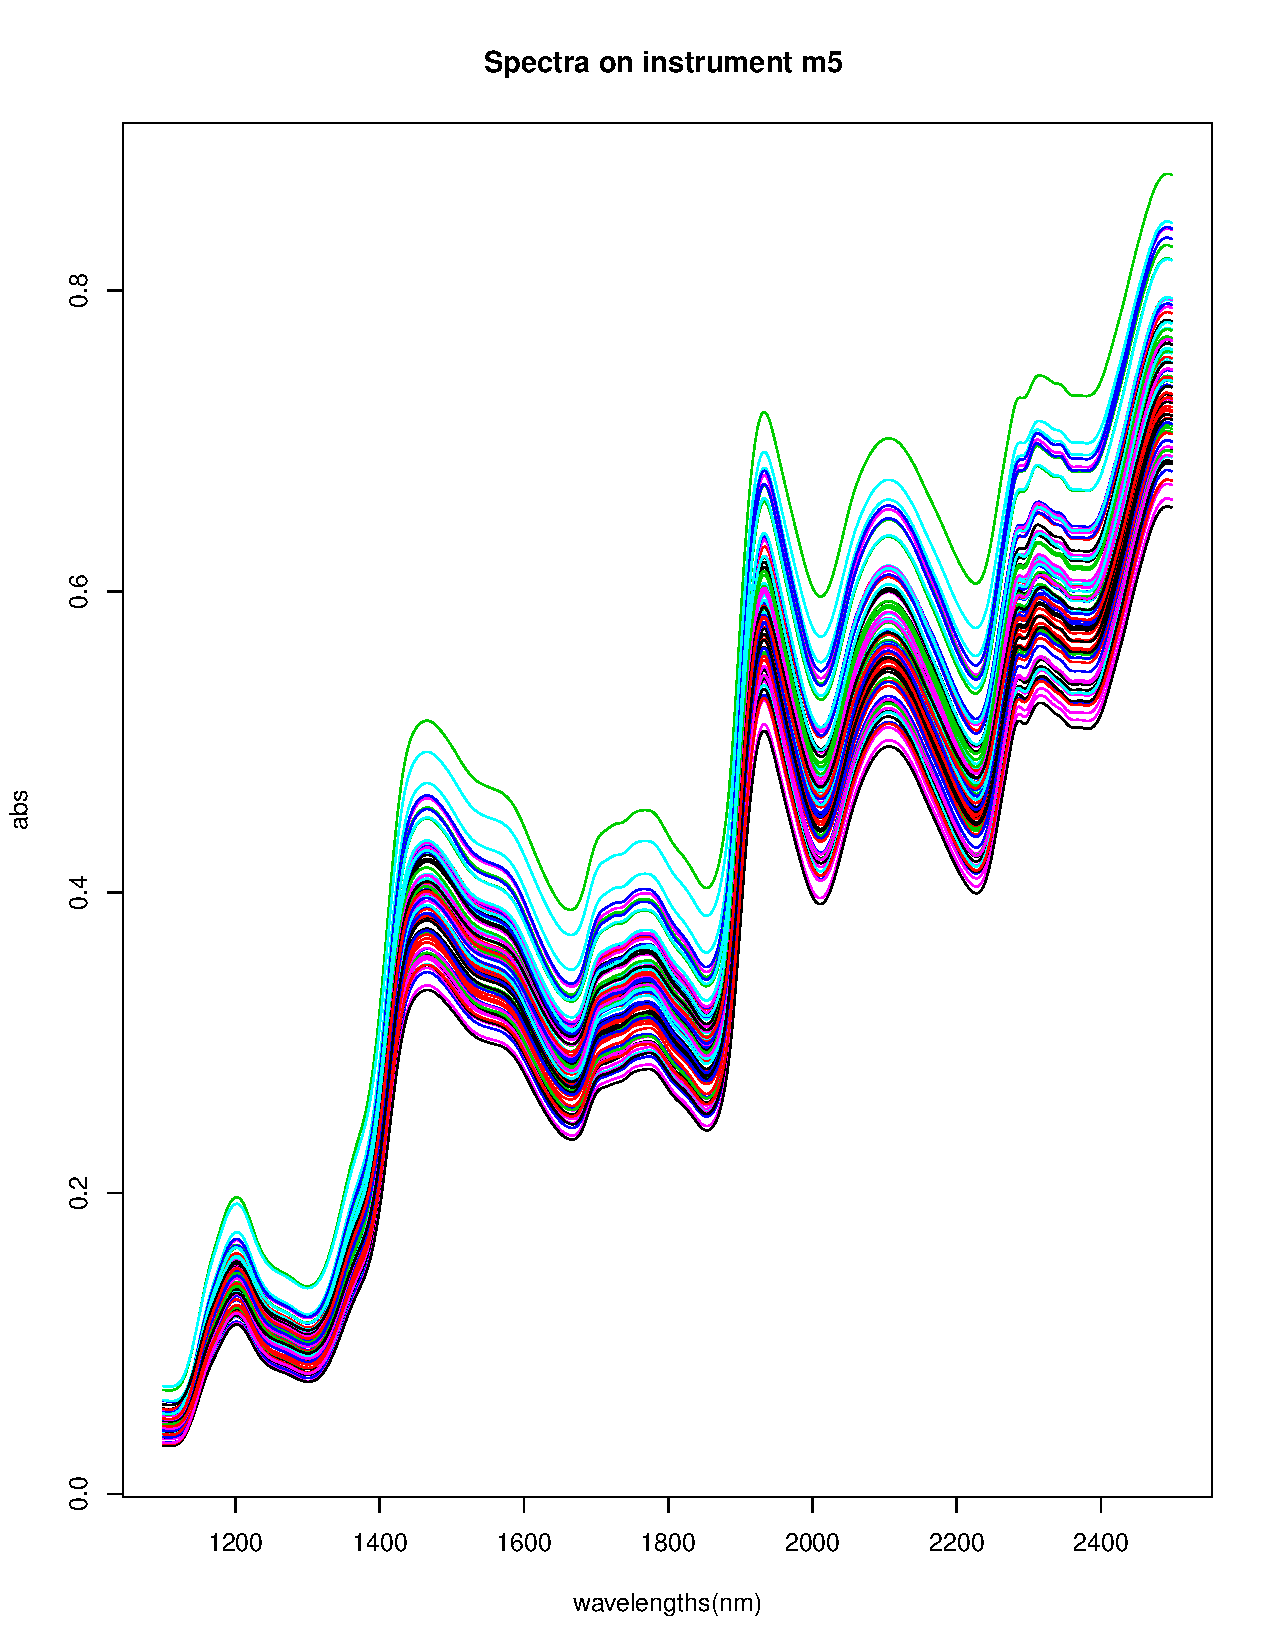
\includegraphics[width=7.5cm, angle=0]{Spectra_on_instrument_m5.pdf}  % width changes size
				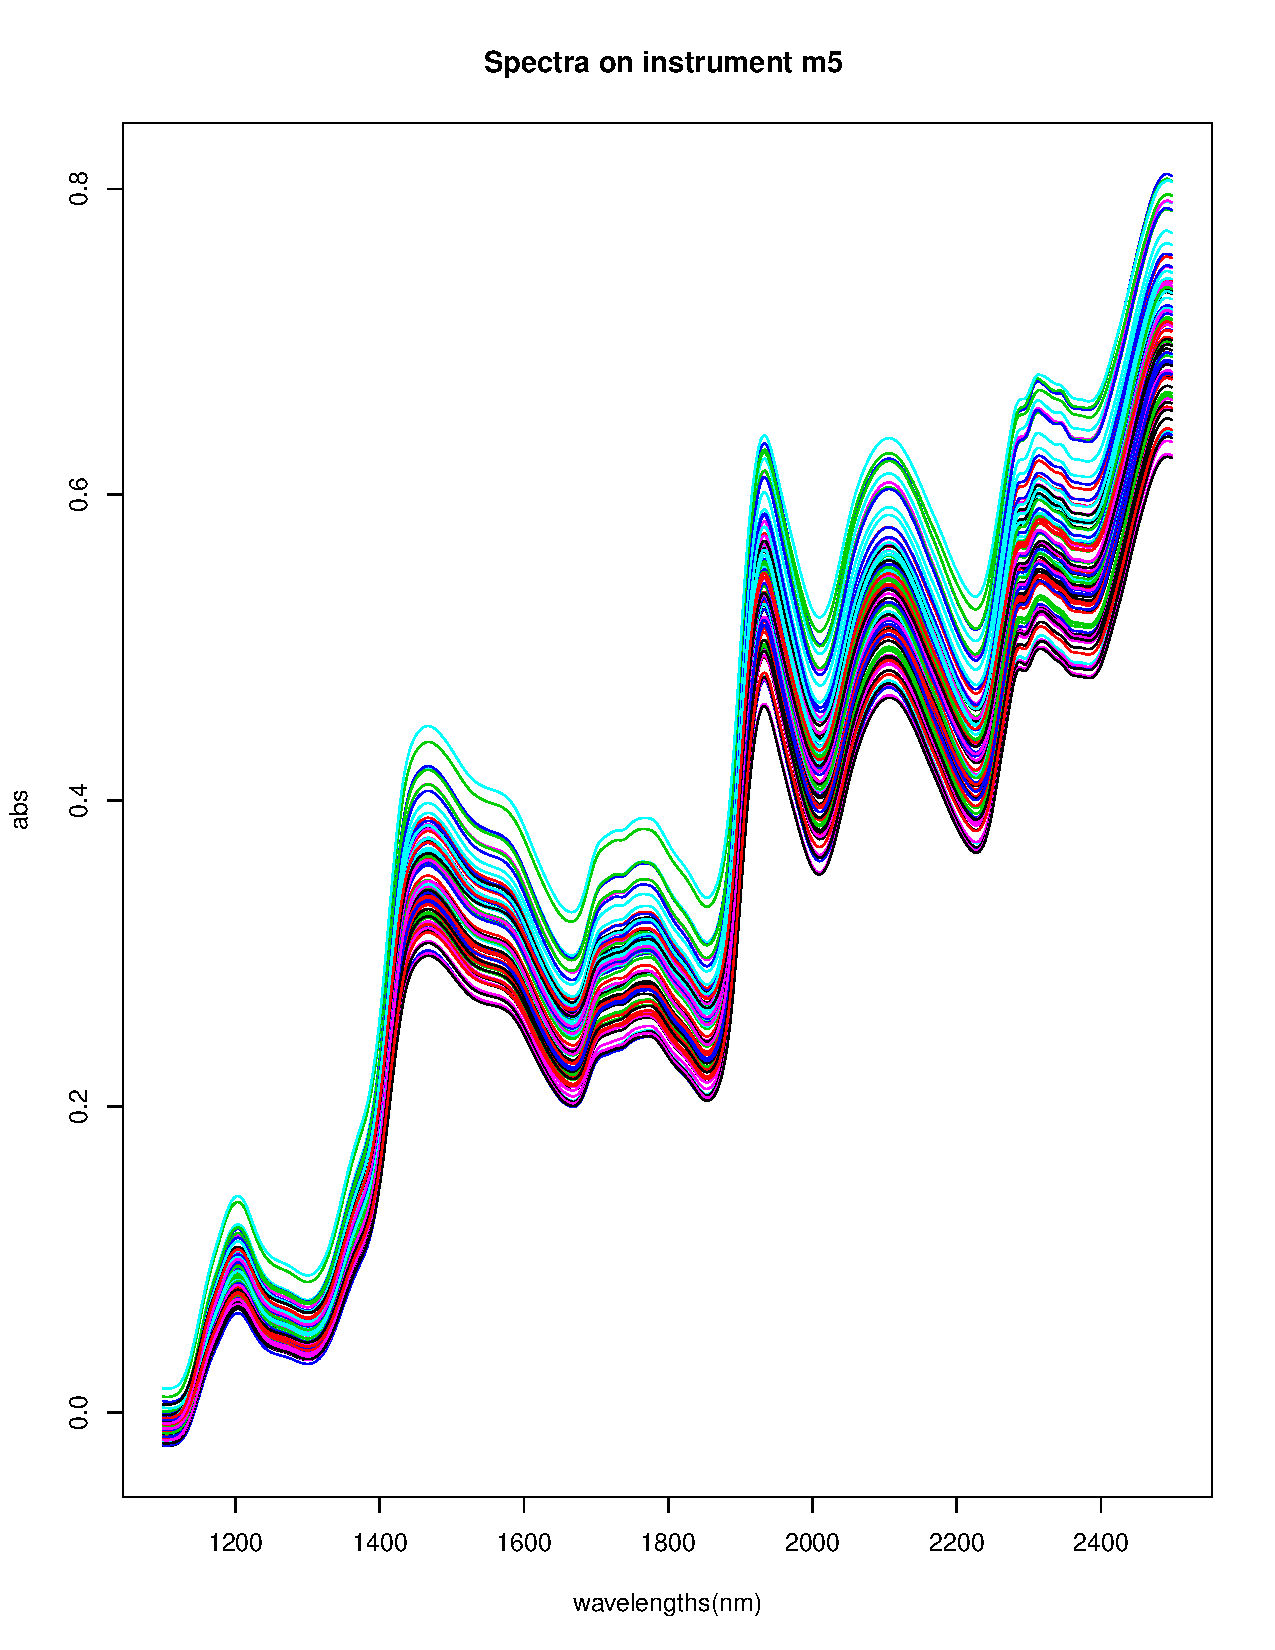
\includegraphics[width=7.5cm, angle=0]{Spectra_on_instrument_mp5.pdf}  % width changes size
		\caption{Spectra on instrument m5 and mp5}          % a meaningful caption
		\label{fig:Spectra_on_instrument_m5}               % label for the figure
	\end{figure}                        % end of figure environment
	
	 Each of these samples also gives the corresponding moisture, oil, protein and starch values. In this dissertation, the spectrum data measured by m5 spectrometers calls as m5. So the same as mp5 and mp6. And one of m5, mp5 and mp6 NIR data will be selected as $X$ in each regression. The value related to the moisture, oil, protein and starch values was considered as the dependent variable $Y$. So $X$ should be one of three 80$\times$700 matrices and $Y$ should be one of four 80$\times$1 vectors.
	  In addition, corn data set will be divided into a calibration set and a prediction set using a random sampling method. Model the calibration set and then predict prediction set. Finally, RMSECV and RMSEP are calculated as the criterion.
	
	Firstly, the effect of each conditions on partial least squares regression (PLSR) is observed by different performance of PLSR based on corn data under different conditions. Then find out as much papers using corn data as possible to compare the results in papers with the results in dissertation. In this way, we can observe whether the new algorithm has a significant improvement compared to PLSR. Finally, the F-test is used to test whether the new method is significantly different from PLS.
	
	

	
	\section{Methodology}
	\label{sec:method}
	
	\subsection{Model Evaluation}
	\label{sec:eva}
	According to the corn data literature, there are several measures that can be used to evaluate the performance of the model.

	1. Root Mean Square Error for Calibration samples (RMSEC) is proposed by \citet{2yun2014strategy}.
	
	2. RMSECV is mentioned by many papers \citep{8ji2015using}. And there are two cross-validation methods. One is leave one out cross-validation (LOOCV), mentioned by \citet{6zheng2015pretreating}. The other is K-fold cross-validation, there are the 3-fold cross-validation \citep{3galvao2007cross}, 10-fold cross-validation \citep{8ji2015using} and so on. The calculation method of RMSECV is as follows:
	
	\begin{equation}
	RMSECV=\sqrt{\frac{1}{n}\sum_{i=1}^{n} (y_i-\hat y_i)^2} 
	\end{equation}
	\begin{conditions}
		n     &  the number of samples\\
		y_i     &   the experimental value of the i-th sample\\   
		\hat y_i &  the predicted value of the i-th sample by cross-validation which  includes removing the set of i-th sample from the calibration set, building a model with the remaining samples, and applying the model to i-th sample
	\end{conditions}
	
	3. The Root Mean Square Error of Prediction (RMSEP) is mentioned by \citet{1su2006partial}. This is a generally accepted method of evaluating models. This approach requires the determination of appropriate cross-validation sets and prediction sets before building PLS model. For example, 60 samples of corn data are used for a cross-validation and the remaining 20 samples are used as predictions \citep{1su2006partial}. Then the cross-validation data is used for modelling, determining the parameters for regression model, such as PLS. After that, the model is applied to the predictive data to calculate the Root Mean Square Error of Prediction (RMSEP). The RMSEP calculation formula is:
	
	\begin{equation}
	RMSEP=\sqrt{\frac{1}{m}\sum_{i=1}^{m} (y_i-\hat y_i)^2}
	\end{equation}
	
	\begin{conditions}
		m     &  the number of prediction sets\\
		y_i     &  the experimental value of the i-th sample in the prediction set \\   
		\hat y_i &  the prediction value of model for the i-th sample
	\end{conditions}
	
	
	4. There are few papers mentioned that $R^2$ is used to measure the model \citep{tatavarti2005assessment}. But this method is also flawed. In some situations, not enough calculation accuracy of the computer will cause the value of $R^2$ to be equal to 1. For example, \citet{deng2016bootstrapping} has this problem and the $R^2$ in PLS model fitting  moisture is equl to 0.9959, but for the CARS, GA-PLS and BOSS model, $R^2$ are all equal to $1.0000 \pm 0.0000$. Hence we can see it hard to distinguish the different between models. So this will not be a good indicator of evaluation.
	
	\subsection{Pre-treatment}
	\label{sec:treat}
	The papers use different pre-treatments of the data, and the results of the model will be very different. For example, \citet{7galvao2008variable} and \citet{8ji2015using} both use M5 to predict the first constituent, and the results are very different. Through the different literatures, the common pretreatment of corn data has the following four types:

	\begin{enumerate}
			
	\item Nothing to deal with \citep{1su2006partial}.
	
	\item Scale the data \citep{4ergon2006reduced}.
	
	\item SavitzkyGolay filter processing on the data \citep{3galvao2007cross}.
	
	\item Delete the outliers. For example \citet{8ji2015using} take out the 75th and 77th corn 
	spectrum from dataset as outliers.
	
	\end{enumerate}
	
	\subsection{Sample splitting}
	\label{splitting}
	The number of samples selected and the method of sample selection will also have an impact on the results of models. The methods of selecting samples are as follows:
	
	\begin{enumerate}
	
	\item A completely random sample \citep{1su2006partial}.
	
	\item Choosing the samples by SPXY method \citep{3galvao2007cross}.
	
	\item Use the Kennard-Stone (K-S) algorithm \citep{zhao2015optimization}.
	
	\item Directly divide the raw data into the first half and the second half, the first half is cross-validation sets, and the second half is prediction set \citep{4ergon2006reduced}.

	\end{enumerate}
	
	The second and third methods will result in the prediction level data being very close to the data of the cross-validation set, which may increase the accuracy of the prediction and reduce the prediction difficulty, so these two methods are not used here. Because in the actual problem, the performance of the algorithm looks better when the two sample sets are too similar, which is not what we want. The last method relies on the sorting of the original data, so the next step is to take a random sampling method to simulate the sample. The selection of samples refers to \citet{5zheng2012stability} and \citet{6zheng2015pretreating}, so the sample size of 20 $\sim$ 70 will be selected as calibration to build the model, and the rest will selected as prediction.
	
	\subsection{Cross-validation}
	\label{cross-validation}
	The cross-validation is to divide the data into n groups. One of group is selected as the prediction set, and the remaining n-1 groups are used as calibration sets, and testing n times. Finally, the average of results of all tests was taken as the cross-validation result. If the selected n is the same as the size of sample, then this method is called leave one out method (LOO), otherwise it is called the k-fold cross-validation. Cross-validation not only improves the reliability of models, but also allows the model to avoid falling into local optimal solutions. Figure \ref{fig:cross-validation} shows the flow of the cross-validation.
	\begin{figure}[h]    % start of figure environment
		\centering           % put the graph(s) in the centre of the page (horizontally)
		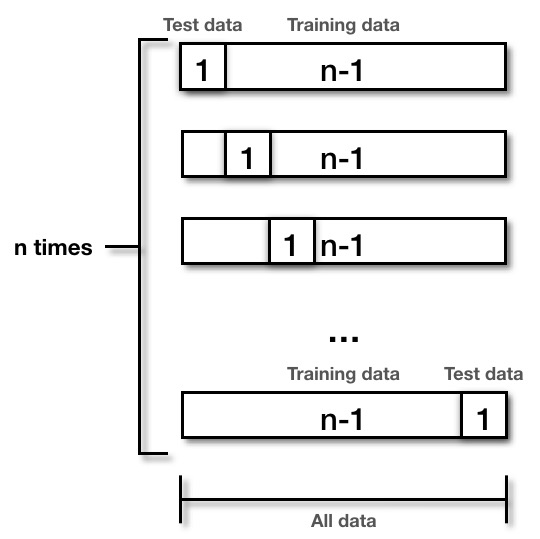
\includegraphics[width=8.5cm, angle=0]{cross-validation.png}  % width changes size
		\vspace*{-0.25cm}    % manual adjustment of vertical spacing
		\caption{The flow of the cross-validation}          % a meaningful caption
		\label{fig:cross-validation}               % label for the figure
	\end{figure}                        % end of figure environment
	
	The choice between LOO and k-fold cross-validation is determined according to the number of samples. When the sample size is small, the LOO is preferred. When the sample size is too large, the k-fold cross-test is preferred. There is an additional reminder here that the difference between LOO and the k-fold cross-validation is not just a difference in computing time. More, when the sample size is too large, LOO may cause over-fitting problems, and the k-fold cross-validation can not only save computational power, but also avoid the over-fitting problem in here. Chapter \ref{sec:Cross-Validation} will discuss the difference.
	
	\subsection{PLS algorithm}
	\label{PLS_al}
	The partial least squares regression (PLS) is a multi-regression technique proposed by \citet{wold1984collinearity}, and it is also the most common statistical method in the research of near-infrared spectroscopy (NIR). Partial least squares regression is similar to principal components analysis (PCA) and is also a factor analysis method. In the modelling  process, it is first necessary to decompose the matrix of spectrum and then extract a few principal components (these variables are called latent variables in PLS) to represent most of the information of original spectrum. Because the spectral data is high-dimensional, the number of independent variables is more than the number of samples, thus it cannot meet the basic assumption of least squares method (OLS). Therefore, it is necessary to extracting the data to some components, and then make the regression. Compared with PCA, PLS not only considers the dimensionality reduction of the independent variables, but also maximizes the covariance between principal components and target variables. In this way, the covariance between the extracted components and the target vector will be the maximum. According to this point, PLS is the improvement and further development of PCA, and the results in many applications also prove that PLS has better performance than PCA.
	
	The process of partial least squares regression is as follows:
	
	The PLS model needs to perform principal component decomposition on the spectral data matrix and the target vector when it is established.
	
	\begin{equation}
	X=TP^T+E 
	\end{equation}
	\begin{equation}
	Y=UQ^T+F
	\end{equation}
	
	Where $T$ and $P$ are the score matrices and the loading matrices of the spectral matrix $X$, respectively. $U$ and $Q$ are the score matrices and the loading matrices of target vector $Y$. $E$ and $F$ are residual matrices of the spectral matrix $X$ and target vector $Y$, respectively, and $T$ and $U$ can perform linear regression as follows:
	
	\begin{equation}
	u_i=t_ib_i
	\label{equ:ui} 
	\end{equation}
	
	Here $t_i$ and $u_i$ are the first column data of $T$ and $U$, respectively.
	
	In the process of establishing partial least squares regression models, the spectral matrix $X$ and the target vector $Y$ are decomposed in an iterative manner. In each iteration, the principal components $t_i$ and $u_i$ of $T$ and $U$ can be obtained separately. Linear regression is performed on $t_i$ and $u_i$ by Equation (\ref{equ:ui}), and then the information explained by $t_i$ and $u_i$ is subtracted from spectral matrices and target vectors, respectively, to obtain the residual matrices. Finally, the residual matrices is brought into the previous iterative process again, which are the spectral matrices and the target vectors in next iteration. This iterative process is terminated by constant iteration until the latent variable of the specified target is obtained. The specific operation flow, pseudocode as follows:
	
	\begin{enumerate}
	
	\item Initialize the score vector $u=Y$.
	
	\item Calculate the weight vector $\omega$ by formula \ref{equ:omega}:
	
	\begin{equation}
	\omega=X'u/(u'u)
	\label{equ:omega} 
	\end{equation}
	
	\item Let $\omega=\omega/\left\|\omega\right\|$.
	
	\item Calculate the spectral score vector $t=X\omega$.
	
	\item Calculate the spectral matrices' loading vector $p=X't/(t't)$.
	
	\item According to the spectral matrix score vector, calculate target vector $q=Y't(t't)$.
	
	\item Let $X=X-tp'$ and $Y=Y-tq$.
	
	\item If the number of extracted latent variables reaches number required by the algorithm, the iteration is terminated, otherwise go back to step 1 and continue the next iteration.
	
	\end{enumerate}
	
	After the iteration process finish, the regression coefficients of the partial least squares regression model (PLSR) are calculated according to the equation \ref{equ:B}.
	\begin{equation}
	B=W(P'W)^{-1}Q
	\label{equ:B} 
	\end{equation}
	
	Finally, the prediction model of the partial least squares regression model is as equation \ref{equ:y_unknow}.
	\begin{equation}
	Y_{unknow}=X_{unknow}B
	\label{equ:y_unknow} 
	\end{equation}
	
	\subsection{Parallel computing}
	\label{parallel}
	
	Parallel computing is the simultaneous calculation of tasks that are broken down into subtasks into multiple cores. There are two computer calculation ways: serial calculations, such as iterative algorithms, and parallel calculations, such as repeated experiments. When an algorithm calculations are all serial tasks, it is completely impossible to use parallel computing. When all the calculations from an algorithm are parallel tasks, then full parallel computing can be used. So, how much parallel computing can improve algorithm, it depends on the proportion of the algorithm's serial computing part and parallel computing part respectively. When there are less serial calculations in algorithm, the more time can be saved by parallel computing. In this dissertation, each partial least square regression process is a serial calculation and cannot be optimized by  parallel computing. However, repeated experiments with partial least squares regression can be optimized using parallel computing.
	
	Because this dissertation is computationally heavy, parallel computing is considered to improve the efficiency of algorithm. Through the analysis of a small amount of experimental data, it is estimated that if a single-core calculation is used, the computation required to complete the whole paper will take about three months to end the calculation. In terms of time, if  dissertation doesn't optimize the algorithm, this is an impossible task to finish dissertation in time.
	
	Parallel computing in R language is divided into two categories, one is implicit parallel computing and the other is explicit parallel computing. Implicit parallel computing hides most of the parallel computing details from the user, and the user does not need to know the specific calculation process. After library the implicit parallel computing related R packages, the system automatically enables parallel computing based on the current resources. The related R package includes "OpenBLAS", "Intel MKL" and "NVIDIA cuBLAS". But the disadvantage of this kind of parallel computing is that the efficiency of the upgrade is extremely limited. The other is explicit parallel computing. Explicit parallel computing requires the user to actively run parallel computing, and actively divide the data and assign tasks. This type of parallel computing can effectively improve the efficiency of the algorithm, but not as friendly as the former. The associated R language explicit parallel package includes "parallel", "foreach", "SupR" and "gpuR". Whether it is implicit parallel computing or parallel computing, parallel computing consumes a lot of memory, and the lazy evaluation programming strategy used by R exacerbates this problem. Therefore, when using parallel computing, you need to allocate enough memory space in advance to the program. This dissertation implements parallel computing through the family of "apply" functions optimized by "parallel" package in R.
	
	The main steps of complete parallel computing process are as follows:
	\begin{enumerate}
	\item  Load the parallel package and calculate the number of available cores. R code is as follows:
	\begin{lstlisting}[language=R]
	library(parallel) 
	clnum <- detectCores()
	\end{lstlisting}
	
	\item Initialize and set up a clustered parallel computing environment.
	
	\begin{lstlisting}[language=R]
	cl <- makeCluster(getOption("cl.cores", clnum))
	\end{lstlisting}
	
	\item Assign copies of packages and variables that need to be used in parallel computing to each core.
	
	\begin{lstlisting}[language=R]
	clusterExport(cl, "RawData")
	\end{lstlisting}
	
	\item Run the algorithm optimized for parallel computing.
Here is the optimized code sample as following:
	
	\begin{lstlisting}[language=R]
	Result <- parSapply(cl, x, my_function)
	\end{lstlisting}
	
	\item Shut down the cluster.
	
	
	\begin{lstlisting}[language=R]
	stopCluster(cl)
	\end{lstlisting}
	
	\end{enumerate}


	
	
	Enable different number of cores and running times as shown in Table \ref{parallel_time}. 
	
		\begin{table}[h]
		\centering
		\begin{tabular}{llllll}
			\hline
			Number of core & 1     & 9     & 18    & 27    & 36    \\ \hline
			Running time (s)  & 97.42 & 68.84 & 58.56 & 55.77 & 54.97 \\ \hline
		\end{tabular}
		\caption{Different number of cores vs. running time of parallel computing and one core means no parallel computing.}
		\label{parallel_time}
	\end{table}
	
	
	Table \ref{parallel_time} shows running time required for the corn data m5 spectrum to perform 5000 partial least squares regression on moisture data. As can be seen from the table, as the number of cores increases, the running time shows a significant downward trend. But when the number of cores exceeds a certain limit, the algorithm improvement through parallel computing is getting smaller and smaller. This is because, when the number of cores is too large, it will take a lot of time to allocate subtasks to the initialization process of each core. But when the amount of calculation becomes larger, parallel computing will show its superiority.
	

	

	
	\subsection{High performance computing (HPC)}
	\label{myriad}
	
	High-performance computers are also often referred to as supercomputers. It is a cluster that is connected by a network of many servers called nodes. A cluster can simultaneously use multiple cores or multiple nodes to run multi-core tasks through a special network. And the reason why use high-performance computers for calculation in this dissertation is as follows.

	\begin{enumerate}
	\item Dissertation needs to run large parallel jobs. Usually, a single-core program needs to run continuously for 6$\sim$12 hours on personal computers every times. The personal computers cannot do anything  while running large parallel jobs, and you need to make sure computers do not encounter any unexpected situations, such as sleep, power outages, and accidental touches on the keyboard. So such a task is an unrealistic job to run locally.

	\item Dissertation needs large quantities of RAM. Because this thesis uses parallel computing so many times, it consumes a lot of computer memory than a single core compute. While personal computers usually have only 16 GB, less than half of the available memory can be allocated to programming. So in terms of memory requirements, personal computers are not good enough.

	\end{enumerate}

	This dissertation uses two high-performance computing systems ,named "Myriad" and "Grace", provided by University College London. "Grace" consists of 684 compute nodes, 10,944 processor cores and over 1 Petabyte high-performance memory, which is the largest and fastest high-performance computing system in the UK university sector.  And there are two ways to run r code through a cluster.

	\begin{enumerate}

	\item Load directly through commands in terminal and then use the R interactively. The codes for starting the R module are as follows.
	
	
	\begin{lstlisting}[language=sh]
	module unload compilers mpi
	module load r/recommended
	R
	\end{lstlisting}
	
	After setting anaconda environment, the interactive operation interface under tmux shell is as figure \ref{fig:R_cluster}.
	
	\begin{figure}[h]    % start of figure environment
	\centering           % put the graph(s) in the centre of the page (horizontally)
	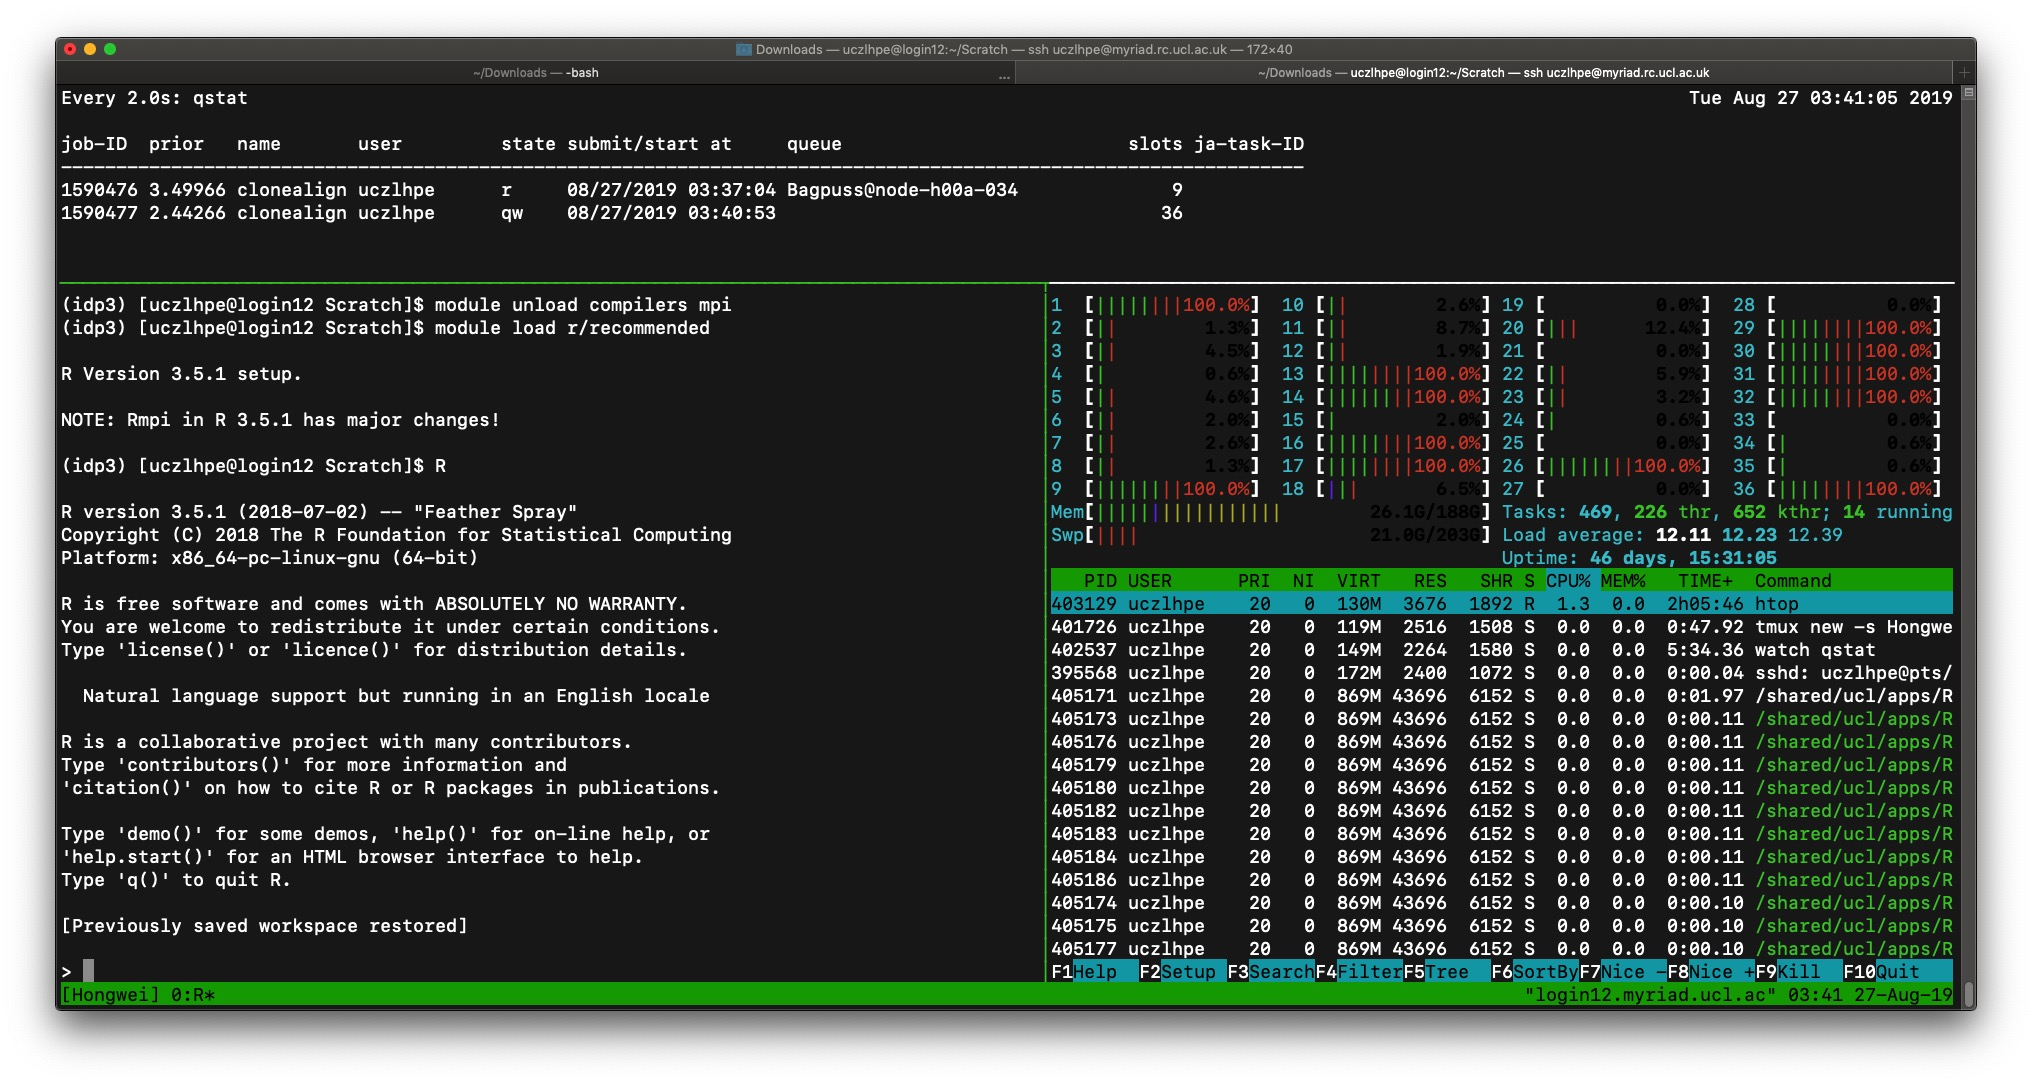
\includegraphics[width=14.5cm, angle=0]{R_cluster.png} % angle changes orientation
	\vspace*{-0.25cm}    % manual adjustment of vertical spacing
	\caption{R interactive operation interface under tmux shell}          % a meaningful caption
	\label{fig:R_cluster}               % label for the figure
	\end{figure}                        % end of figure environment
	
	
	\item Submit the task to the cluster through a batch job. These functions can be implemented through a runscript. Among this R runscript, the following variables need to be set in script:  required max wallclock time, required max memory, and required number of cores when run. There are also other additional functions, such as output path, or sending a message to mailbox when the code finishes running. These functions can be implemented through scripts. Finally, enter the command, start R module, and run the specified R file.
	
	Simplified runscript is shown below.
	
	\begin{lstlisting}[language=sh]
#!/bin/bash -l
#$ -S /bin/bash                          #Set type of shell
#$ -pe mpi 36                            #Set number of cores
#$ -l tmpfs=30G                          #Set max memory
#$ -l h_rt=48:0:0                        #Set max wallclock time
#$ -wd /lustre/scratch/scratch/uczlhpe/output
                                         #Set working path
#$ -m eas                                #Set email notification
#$ -M xxx@ucl.ac.uk                      #Set email address

module unload compilers
module unload mpi
module load r/recommended
R CMD BATCH run.R                        #Run R code
	\end{lstlisting}
	
After completing the runscript, it can use "qsub" to submit this script into remote server queue and wait for it to run.
	
	\end{enumerate}
	
	Both methods have advantages and disadvantages.
	The first method requires online wait, but the submitted task can be run immediately, and is suitable for use in program testing or when running a single program. In the second method, although it takes a while to run the code, when running a large number of serial programs and large parallel programs, it is a more sensible choice to submit the script to the cluster for calculation. In contrast, the advantage of clustering can be found not only in a more stable and better configuration than PC. Using a cluster also allows you to run multiple files at once, and a cluster can have multiple nodes running on multiple files at the same time. By disassembling the computing tasks and submitting them to the cluster in batches, the single-core calculation that takes up to three months to complete can be completed in just one week.
	
	\section{Result and discussion}
	\label{sec:result}
	
	\subsection{Loop times}
	\label{sec:Loop times}
	
	Set different loop times and repeat PLSR to calculate how many loop times are needed to get stable results. Too small a number of cycles will result in very unstable results and large standard deviations. However, because of the limitations of computer, there are also upper limits on the number of loop times. If the program loops too many times, it will require a unimaginable long runtime.
	
	First, 40 samples were randomly selected as calibration set 40 samples as prediction set. Then make 10 as the number of component. Calculate the corresponding RMSECV and RMSEP. Then continue to cycle this process, get the figure of RMSECV and RMSEP based on different loop times. Through above steps, the  figure \ref{fig:sd_RMSECV_RMSEP} based on the partial least squares result under different cycle times can be obtained. Left graph of figure \ref{fig:sd_RMSECV_RMSEP} is RMSECV and the right boxplot is RMSEP.
	
	\begin{figure}[]    % start of figure environment
		\centering           % put the graph(s) in the centre of the page (horizontally)
		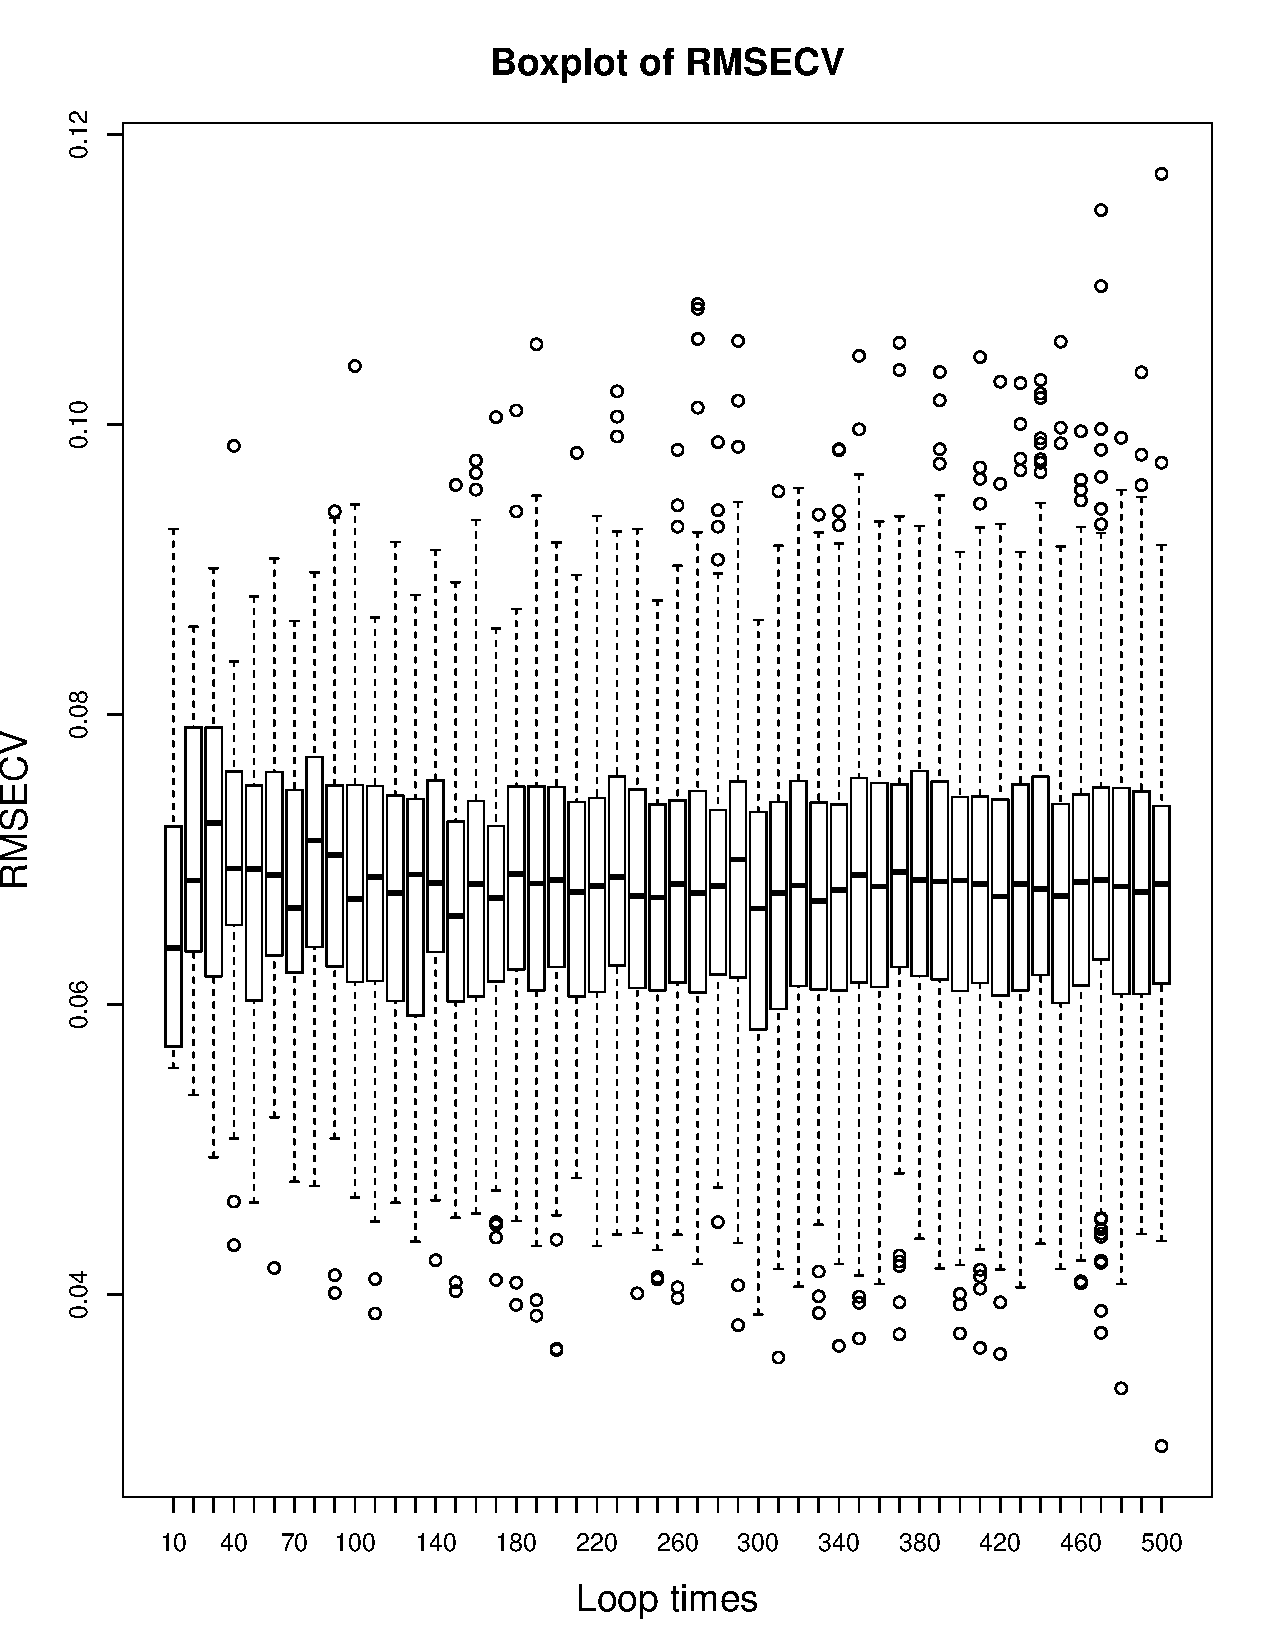
\includegraphics[width=5.5cm, angle=0]{boxplot_RMSECV_loop_times_500.pdf}  % width changes size
		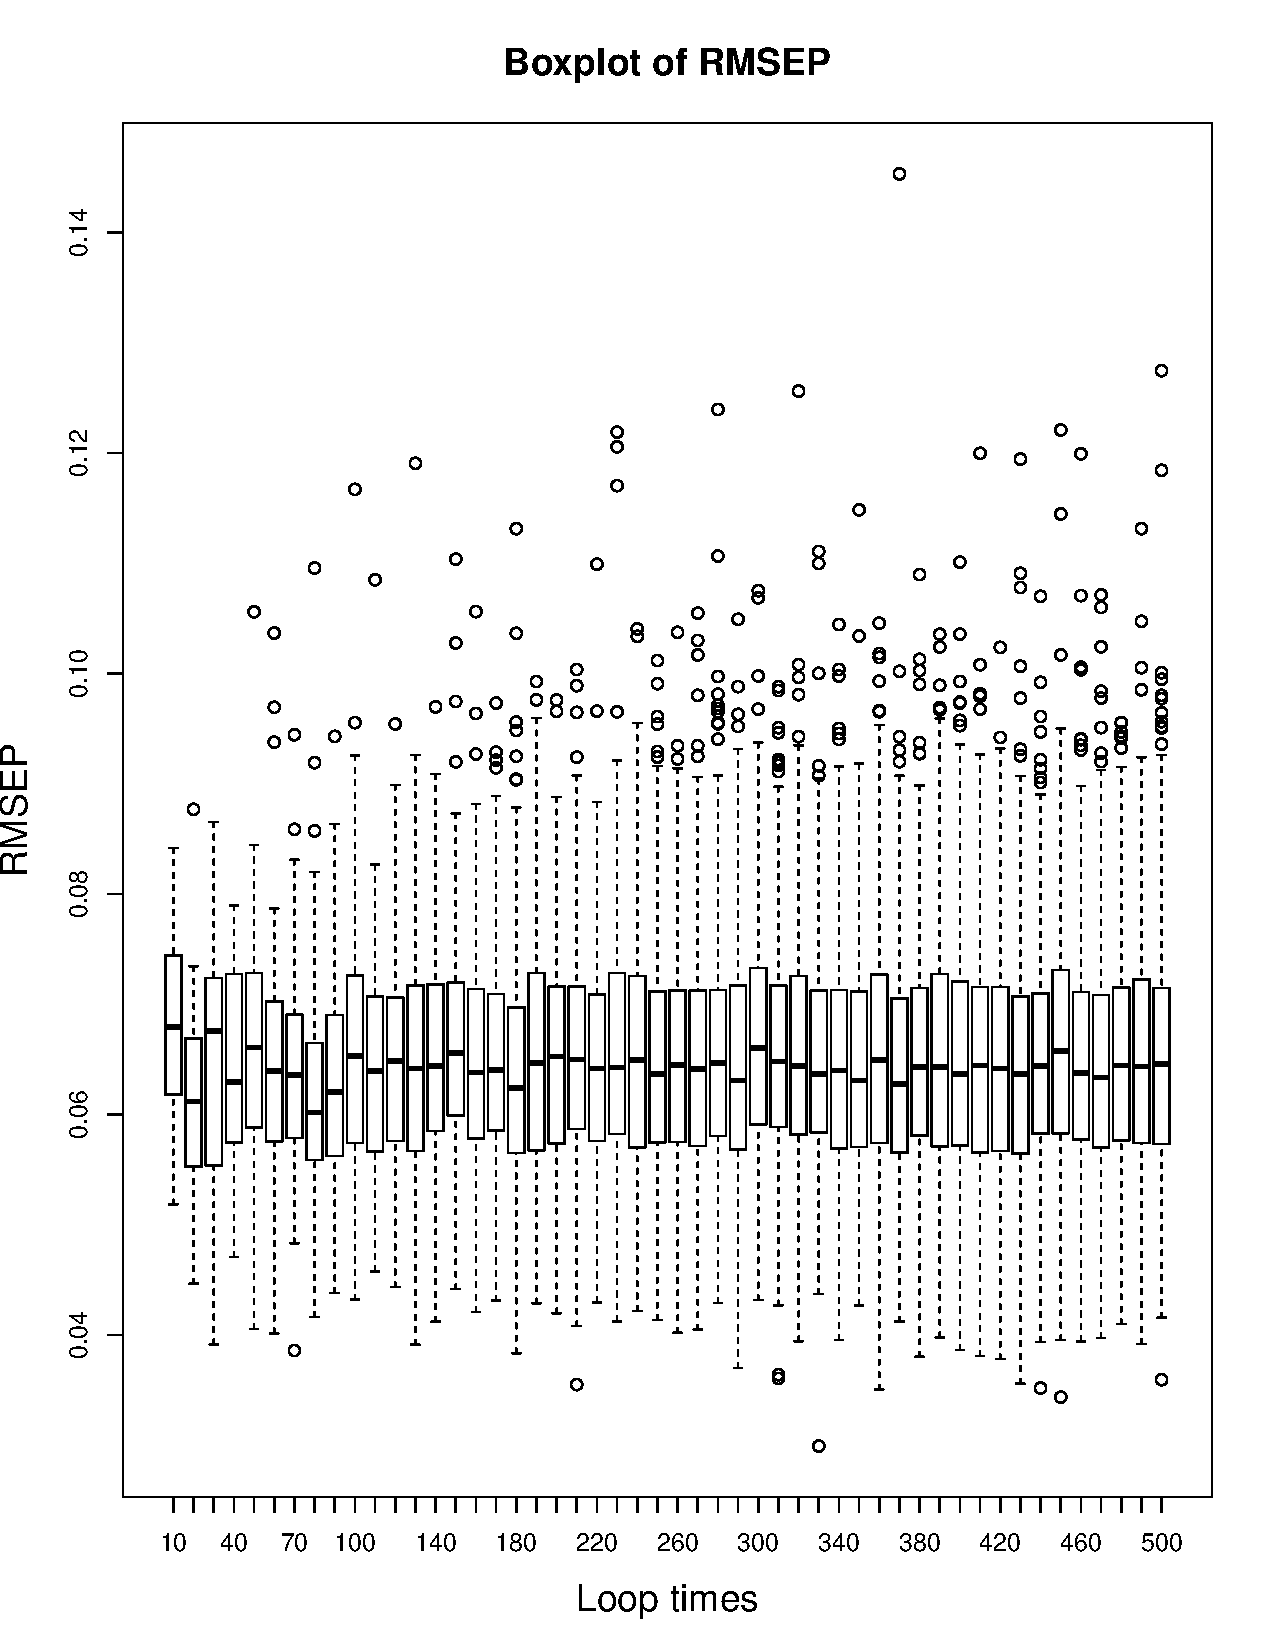
\includegraphics[width=5.5cm, angle=0]{boxplot_RMSEP_loop_times_500.pdf} % angle changes orientation
		%\vspace*{-0.25cm}    % manual adjustment of vertical spacing
		\caption{The boxplot of RMSECV and RMSEP from PLSR of oil on m5 under different loop times}          % a meaningful caption
		\label{fig:sd_RMSECV_RMSEP}               % label for the figure
	\end{figure}                        % end of figure environment
	
	
	 Figure \ref{fig:sd_RMSECV_RMSEP} shows that when the number of loops is too small, the results are not stable enough. When the number of cycles is less than 40, the result shows a significant deviation. But this table does not show how much the number of loops is appropriate. Therefore, the standard deviation plots based on loop times is made for before PLSR result. Figure \ref{fig:sd_RMSECV_loop_times_500} shows the standard deviations of RMSECV and RMSEP from PLSR of oil on m5 spectrum under different loop times.
	 
	 
	\begin{figure}[]    % start of figure environment
		\centering           % put the graph(s) in the centre of the page (horizontally)
		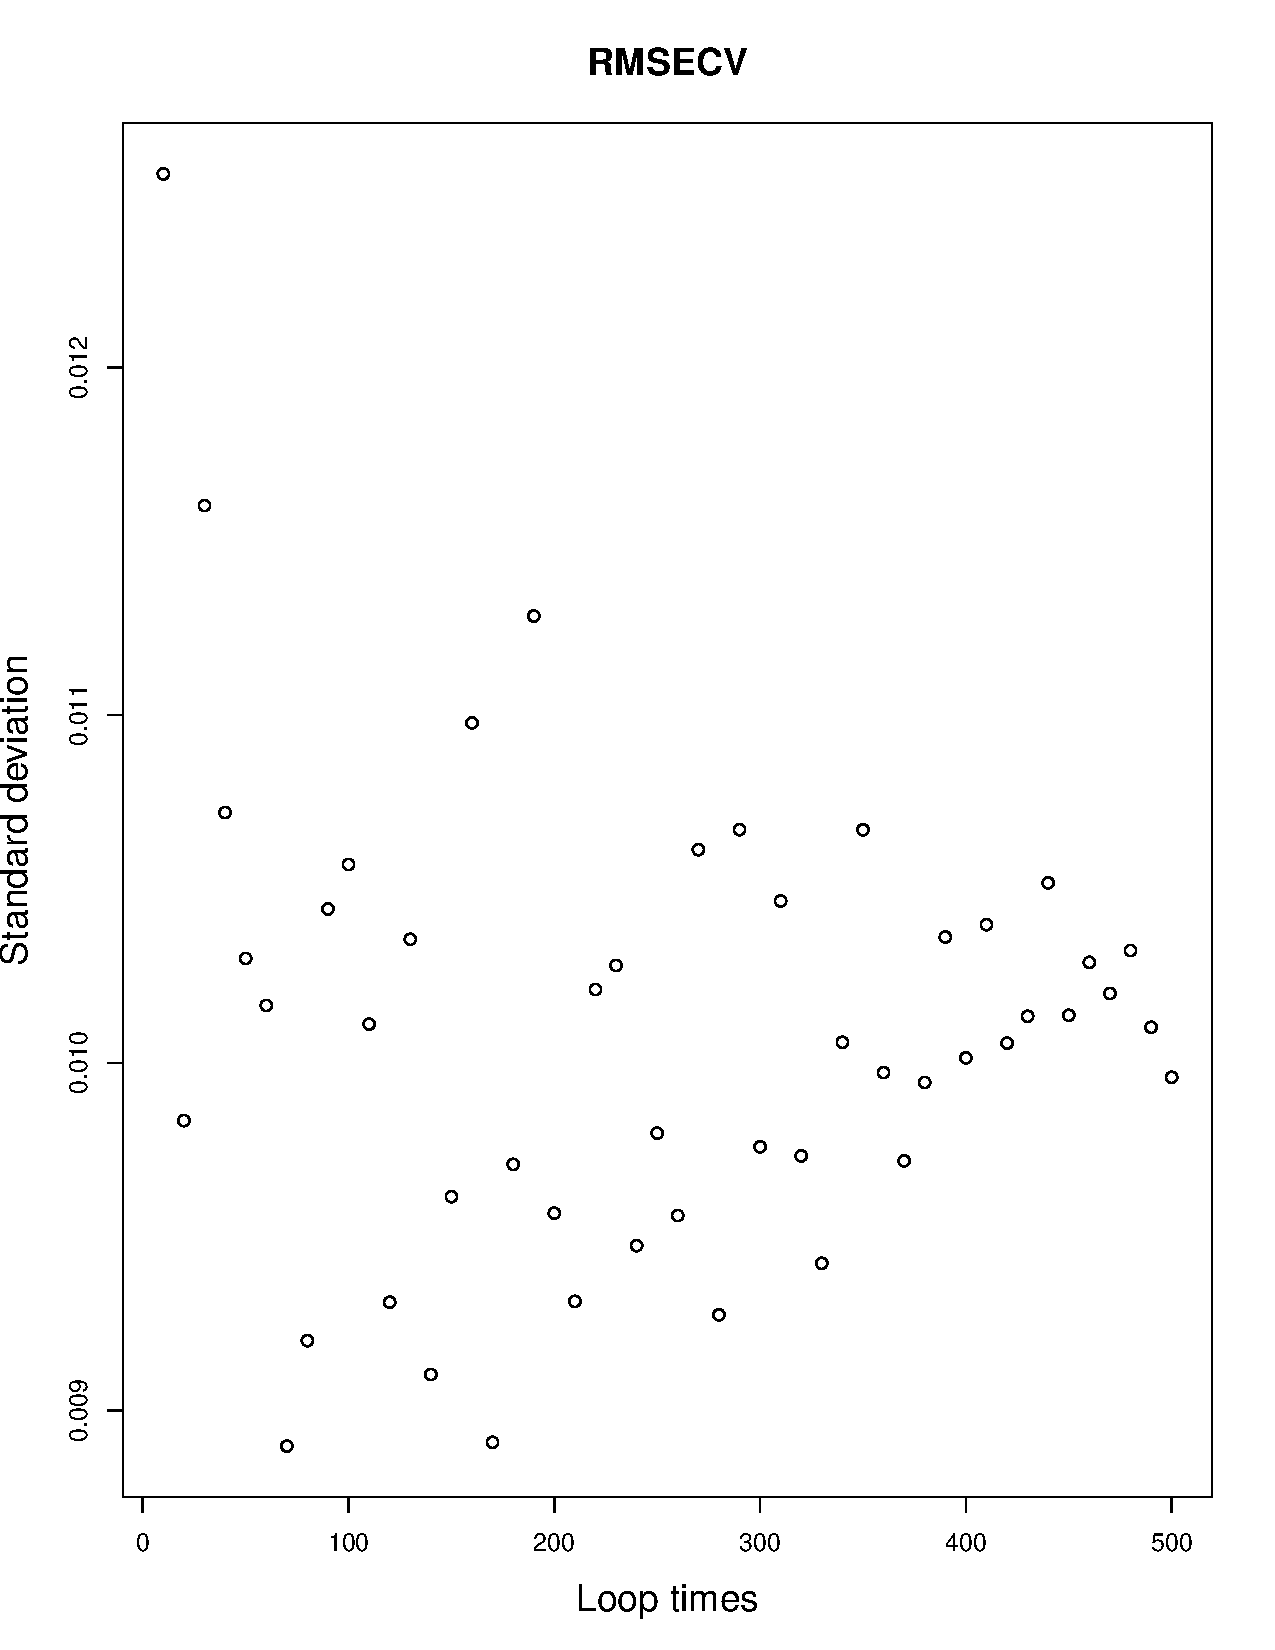
\includegraphics[width=5.5cm, angle=0]{sd_RMSECV_loop_times_500.pdf}  % width changes size
		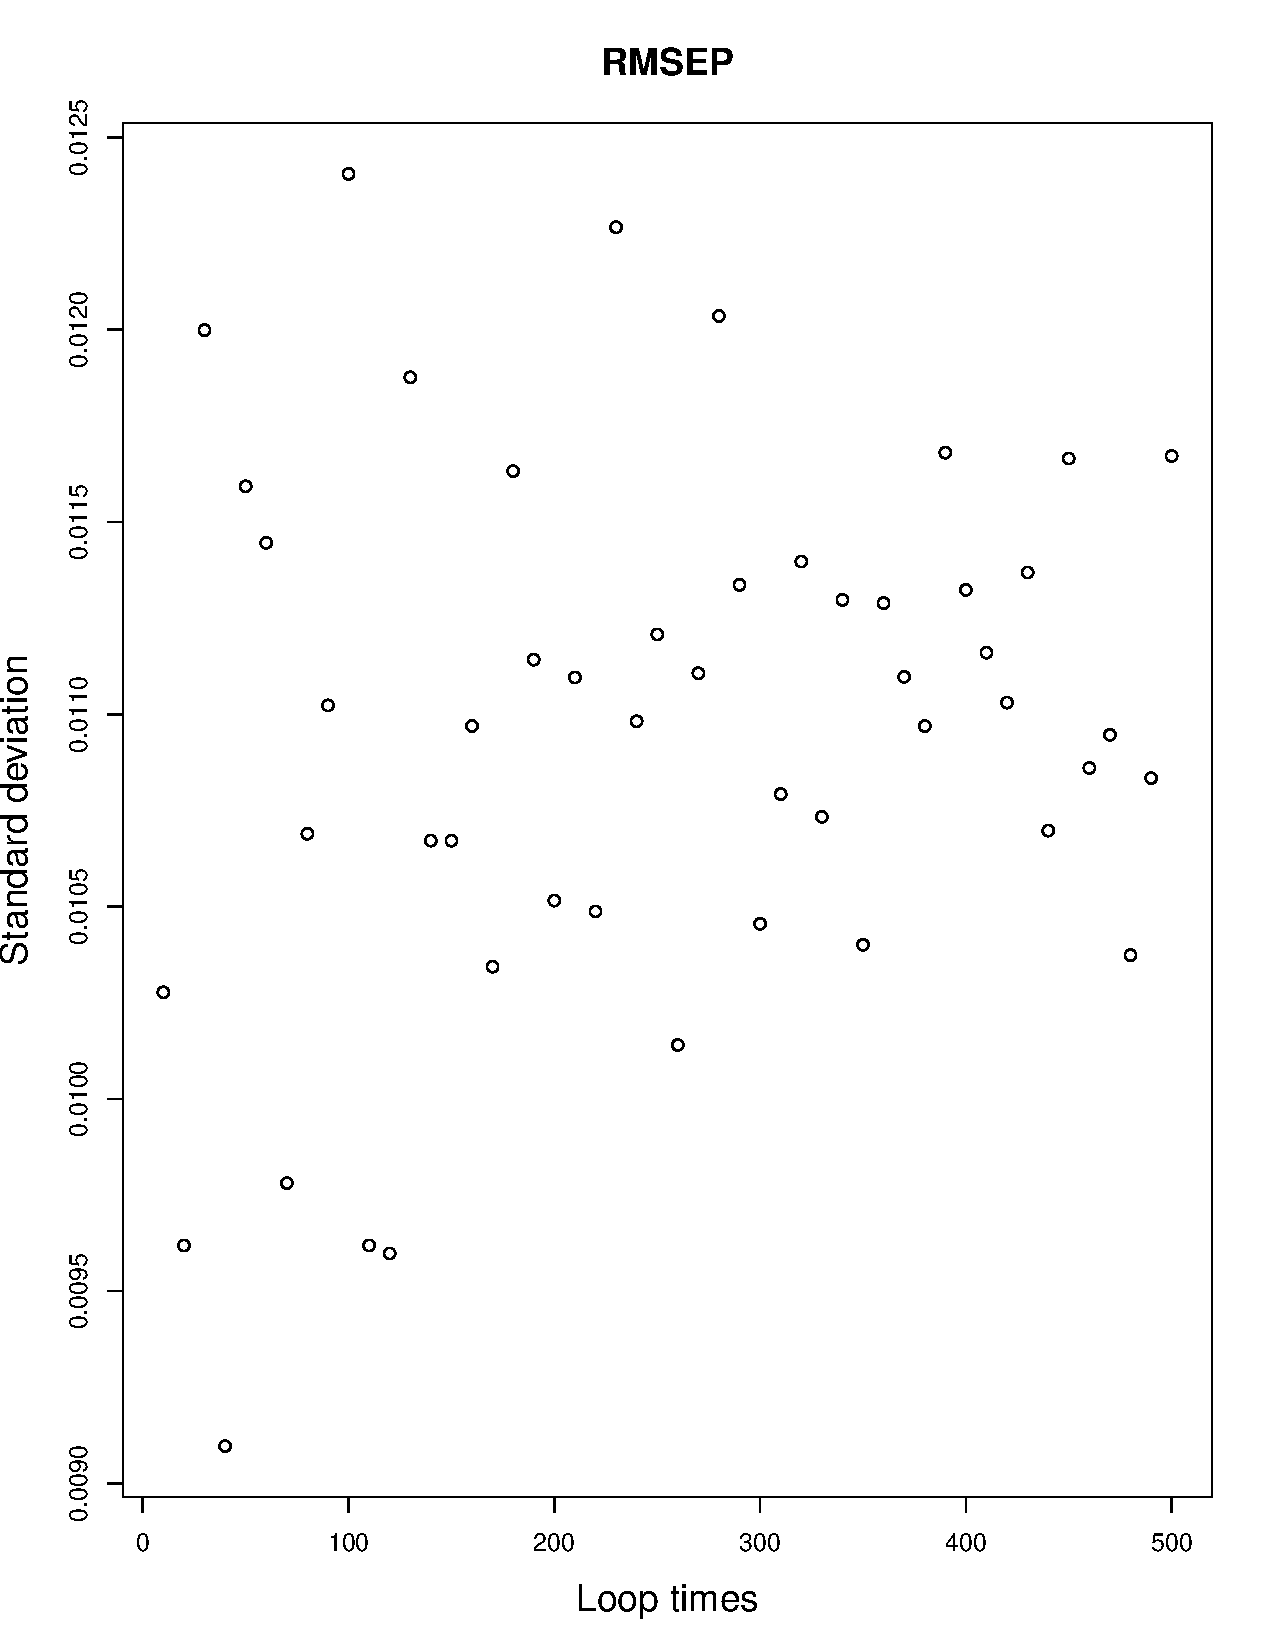
\includegraphics[width=5.5cm, angle=0]{sd_RMSEP_loop_times_500.pdf} % angle changes orientation
		%\vspace*{-0.25cm}    % manual adjustment of vertical spacing
		\caption{The standard deviation of RMSECV and RMSEP from PLSR of oil on m5 under different loop times}          % a meaningful caption
		\label{fig:sd_RMSECV_loop_times_500}               % label for the figure
	\end{figure}                        % end of figure environment
	
	
	Figure \ref{fig:sd_RMSECV_loop_times_500} shows that the standard deviations of RMSECV will decrease as the loop times increases. The RMSEP standard deviations will decrease with the increase of the loop times, and then tend to be stable. Through figure \ref{fig:sd_RMSECV_loop_times_500} it is easy to see that the loop times is around 350, and the standard deviations of RMSEP will show the stable trends. Hence the number of loop times should be set 40$\sim$350 times to get a stable PLSR result. Because less than 40 the results will show a big fluctuation and there are not different results for the more than 350 loop times.
	
	\subsection{Number of samples}
	\label{sec:Number of Samples}
	
	
	
	\subsection{Number of components}
	\label{sec:Number of Components}
	
	\subsection{Pre-treatment}
	\label{sec:Pre-treatment}
	
	\subsection{Cross-validation}
	\label{sec:Cross-Validation}
	
	\subsection{Compare with papers}
	\label{sec:Compare with papers}
	
	
	
	\begin{landscape}
		
		\begin{table}[]
			\begin{tabular}{ll}
				\hline
				Number & Paper's title                                                                                                                          \\ \hline
				1      & A Partial Least Squares‐Based Consensus Regression Method for the Analysis of Near‐Infrared Complex Spectral Data of Plant Samples \\
				2      & A strategy that iteratively retains informative variables for selecting optimal variable subset in multivariate calibration            \\
				3      & Reduced PCR/PLSR models by subspace projections                                                                                        \\
				4      & Stability competitive adaptive reweighted sampling (SCARS) and its applications to multivariate calibration of NIR spectra             \\
				5      & Cross-validation for the selection of spectral variables using the successive projections algorithm                                    \\
				6      & A variable elimination method to improve the parsimony of MLR models using the successive projections algorithm                        \\
				7      & Pretreating near infrared spectra with fractional order Savitzky–Golay differentiation (FOSGD)                                       \\
				8      & Using consensus interval partial least square in near infrared spectra analysis                                                        
			\end{tabular}
			\caption{Papers and related numbers}
			\label{tab:papers}
		\end{table}
		
	\end{landscape}
	
	\begin{landscape}
		
		%Table \ref{tab:moisture} is the regression for moisture.
		% Please add the following required packages to your document preamble:
		% \usepackage{multirow}
		\begin{table}[]
			\begin{tabular}{llllllllllllllll}
				\cline{1-13}
				\multicolumn{1}{c}{\multirow{2}{*}{Paper}} & \multicolumn{1}{c}{\multirow{2}{*}{\begin{tabular}[c]{@{}c@{}}Data\\ set\end{tabular}}} & \multicolumn{1}{c}{\multirow{2}{*}{\begin{tabular}[c]{@{}c@{}}Pre-\\ treatment\end{tabular}}} & \multirow{2}{*}{\begin{tabular}[c]{@{}l@{}}Calibration\\ set\end{tabular}} & \multirow{2}{*}{\begin{tabular}[c]{@{}l@{}}Number of\\ Components\end{tabular}} & \multicolumn{2}{c}{Moisture} &  & \multicolumn{2}{c}{PLS in papers} &  & \multicolumn{2}{c}{Developed method} &  &  &  \\ \cline{6-7} \cline{9-10} \cline{12-13}
				\multicolumn{1}{c}{} & \multicolumn{1}{c}{} & \multicolumn{1}{c}{} &            &    & RMSECV           & RMSEP           &   & RMSECV & RMSEP  &   & RMSECV  & RMSEP   &   &   &   \\ \cline{1-13}
				1                    & mp6                  & None                 & 60(LOO)    & 10 &                  & 0.148(0.0213)   &   &        & 0.159  &   &         & 0.139   &   &   &   \\
				2                    & m5                   & None                 & 64(5-fold) & 10 & 0.0152(0.000739) & 0.0202(0.00319) &   & 0.0149 & 0.0201 &   & 0.00026 & 0.00035 &   &   &   \\
				3                    & m5                   & Scale                & 40(LOO)    & 12 &                  & 0.0231(0.00443) &   &        & 0.3506 &   &         & 0.3485  &   &   &   \\
				3                    & mp5                  & Scale                & 40(LOO)    & 12 &                  & 0.159(0.0178)   &   &        & 0.3506 &   &         & 0.3485  &   &   &   \\
				4                    & mp5                  & Scale                & 40(LOO)    & 10 &                  & 0.405(0.0467)   &   &        & 0.357  &   &         & 0.265   &   &   &   \\
				5                    & m5                   & SG(1,2,13)           & 60(3-fold) & 5  &                  & 0.0547(0.00942) &   &        & 0.040  &   &         & 0.012   &   &   &   \\
				6                    & m5                   & SG(1,2,21)           & 60(LOO)    & 6  &                  & 0.0396(0.00625) &   &        & 0.045  &   &         & 0.019   &   &   &   \\
				8                    & m5                   & Delete 75 , 77       & 52(LOO)    & 10 & 0.0221(0.0018)   & 0.0194(0.00298) &   & 0.0124 & 0.0157 &   & 0.0047  & 0.0056  &   &   &   
			\end{tabular}
			
			\caption{regression of moisture.The values in parentheses corresponds to the cross-validation type in calibration set and standard deviation in moisture.}
			\label{tab:moisture}
		\end{table}
		
		
		
		

		
		%Table \ref{tab:oil} is the regression for Oil.
		% Please add the following required packages to your document preamble:
		% \usepackage{multirow}
		\begin{table}[]
			
			\begin{tabular}{llllllllllllllll}
				\cline{1-13}
				\multicolumn{1}{c}{\multirow{2}{*}{Paper}} & \multicolumn{1}{c}{\multirow{2}{*}{\begin{tabular}[c]{@{}c@{}}Data\\ set\end{tabular}}} & \multicolumn{1}{c}{\multirow{2}{*}{\begin{tabular}[c]{@{}c@{}}Pre-\\ treatment\end{tabular}}} & \multirow{2}{*}{\begin{tabular}[c]{@{}l@{}}Calibration\\ set\end{tabular}} & \multirow{2}{*}{\begin{tabular}[c]{@{}l@{}}Number of\\ Components\end{tabular}} & \multicolumn{2}{c}{Oil} &  & \multicolumn{2}{c}{PLS in papers} &  & \multicolumn{2}{c}{Developed method} &  &  &  \\ \cline{6-7} \cline{9-10} \cline{12-13}
				\multicolumn{1}{c}{} & \multicolumn{1}{c}{} & \multicolumn{1}{c}{} &            &    & RMSECV          & RMSEP           &   & RMSECV & RMSEP  &   & RMSECV & RMSEP          &         &    &                 \\ \cline{1-13}
				1                    & mp6                  & None                 & 60(LOO)    & 10 &                 & 0.0991(0.0161)  &   &        & 0.107  &   &        & 0.0948         &         &    &                 \\
				3                    & m5                   & Scale                & 40(LOO)    & 14 &                 & 0.396(0.0665)   &   &        & 0.6912 &   &        & 0.6902         &         &    &                 \\
				3                    & mp5                  & Scale                & 40(LOO)    & 14 &                 & 0.694(0.095)    &   &        & 0.6912 &   &        & 0.6902         &         &    &                 \\
				5                    & m5                   & SG(1,2,13)           & 60(3-fold) & 12 &                 & 0.0329(0.00672) &   &        & 0.029  &   &        & 0.022          &         &    &                 \\
				6                    & m5                   & SG(1,2,21)           & 60(LOO)    & 10 &                 & 0.0505(0.0103)  &   &        & 0.028  &   &        & 0.030          &         &    &                 \\
				7                    & m5                   & SG(0,2,13)           & 64(5-fold) & 7  & 0.0827(0.00419) & 0.0716(0.0116)  &   & 0.0729 & 0.0855 &   &        & 0.0400         &         &    &                 \\
				7                    & m5                   & SG(1,2,13)           & 64(5-fold) & 7  & 0.0639(0.00357) & 0.0548(0.012)   &   & 0.0577 & 0.0682 &   & 0.0363 & 0.0400         &         &    &                 \\
				7                    & m5                   & SG(2,2,13)           & 64(5-fold) & 7  & 0.0480(0.00312) & 0.0368 (0.0088) &   & 0.0370 & 0.0397 &   & 0.0363 & 0.0400         &         &    &                 \\
				8                    & m5                   & Delete 75 , 77       & 52(LOO)    & 10 & 0.0651(0.00662) & 0.0604(0.00876) &   & 0.0613 & 0.0673 &   & 0.0483 & 0.0546         &         &    &                 
			\end{tabular}
			
			\caption{regression of oil. The values in parentheses corresponds to the cross-validation type in calibration set and standard deviation in moisture.}
			\label{tab:oil}
		\end{table}

		%Table \ref{tab:protein} is the regression for protein.
		% Please add the following required packages to your document preamble:
		% \usepackage{multirow}
		\begin{table}[]
			\begin{tabular}{llllllllllllllll}
				\cline{1-13}
				\multicolumn{1}{c}{\multirow{2}{*}{Paper}} & \multicolumn{1}{c}{\multirow{2}{*}{\begin{tabular}[c]{@{}c@{}}Data\\ set\end{tabular}}} & \multicolumn{1}{c}{\multirow{2}{*}{\begin{tabular}[c]{@{}c@{}}Pre-\\ treatment\end{tabular}}} & \multirow{2}{*}{\begin{tabular}[c]{@{}l@{}}Calibration\\ set\end{tabular}} & \multirow{2}{*}{\begin{tabular}[c]{@{}l@{}}Number of\\ Components\end{tabular}} & \multicolumn{2}{c}{Protein} &  & \multicolumn{2}{c}{PLS in papers} &  & \multicolumn{2}{c}{Developed method} &  &  &  \\ \cline{6-7} \cline{9-10} \cline{12-13}
				\multicolumn{1}{c}{} & \multicolumn{1}{c}{} & \multicolumn{1}{c}{} &            &    & RMSECV           & RMSEP         &   & RMSECV & RMSEP  &   & RMSECV & RMSEP  &   &   &   \\ \cline{1-13}
				1                    & mp6                  & None                 & 60(LOO)    & 10 &                  & 0.141(0.0203) &   &        & 0.150  &   &        & 0.145  &   &   &   \\
				3                    & m5                   & Scale                & 40(LOO)    & 8  &                  & 0.349(0.051)  &   &        & 0.4466 &   &        & 0.4349 &   &   &   \\
				3                    & mp5                  & Scale                & 40(LOO)    & 8  &                  & 0.37(0.0485)  &   &        & 0.4466 &   &        & 0.4349 &   &   &   \\
				5                    & m5                   & SG(1,2,13)           & 60(3-fold) & 6  &                  & 0.107(0.0195) &   &        & 0.119  &   &        & 0.040  &   &   &   \\
				6                    & m5                   & SG(1,2,21)           & 60(LOO)    & 7  &                  & 0.102(0.0186) &   &        & 0.110  &   &        & 0.033  &   &   &   \\
				8                    & m5                   & Delete 75 , 77       & 52(LOO)    & 13 & 0.119 ( 0.0155 ) & 0.11(0.0169)  &   & 0.1080 & 0.1353 &   & 0.0429 & 0.0846 &   &   &   
			\end{tabular}
			
			\caption{regression of protein. The values in parentheses corresponds to the cross-validation type in calibration set and standard deviation in moisture.}
			\label{tab:protein}
		\end{table}

		%Table \ref{tab:starch} is the regression for starch.
		% Please add the following required packages to your document preamble:
		% \usepackage{multirow}
		\begin{table}[]
			\begin{tabular}{llllllllllllllll}
				\cline{1-13}
				\multicolumn{1}{c}{\multirow{2}{*}{Paper}} & \multicolumn{1}{c}{\multirow{2}{*}{\begin{tabular}[c]{@{}c@{}}Data\\ set\end{tabular}}} & \multicolumn{1}{c}{\multirow{2}{*}{\begin{tabular}[c]{@{}c@{}}Pre-\\ treatment\end{tabular}}} & \multirow{2}{*}{\begin{tabular}[c]{@{}l@{}}Calibration\\ set\end{tabular}} & \multirow{2}{*}{\begin{tabular}[c]{@{}l@{}}Number of\\ Components\end{tabular}} & \multicolumn{2}{c}{Starch} &  & \multicolumn{2}{c}{PLS in papers} &  & \multicolumn{2}{c}{Developed method} &  &  &  \\ \cline{6-7} \cline{9-10} \cline{12-13}
				\multicolumn{1}{c}{} & \multicolumn{1}{c}{} & \multicolumn{1}{c}{} &            &    & RMSECV         & RMSEP         &   & RMSECV & RMSEP  &   & RMSECV & RMSEP          &         &    &               \\ \cline{1-13}
				1                    & mp6                  & None                 & 60(LOO)    & 10 &                & 0.35(0.056)   &   &        & 0.370  &   &        & 0.358          &         &    &               \\
				3                    & m5                   & Scale                & 40(LOO)    & 9  &                & 0.393(0.0736) &   &        & 0.5010 &   &        & 0.4443         &         &    &               \\
				3                    & mp5                  & Scale                & 40(LOO)    & 9  &                & 0.513(0.0779) &   &        & 0.5010 &   &        & 0.4443         &         &    &               \\
				5                    & m5                   & SG(1,2,13)           & 60(3-fold) & 6  &                & 0.239(0.0449) &   &        & 0.196  &   &        & 0.100          &         &    &               \\
				6                    & m5                   & SG(1,2,21)           & 60(LOO)    & 5  &                & 0.258(0.0453) &   &        & 0.228  &   &        & 0.101          &         &    &               \\
				7                    & m5                   & SG(0,2,13)           & 64(5-fold) & 8  & 0.333(0.0226)  & 0.283(0.0624) &   & 0.312  & 0.214  &   & 0.240  & 0.219          &         &    &               \\
				7                    & m5                   & SG(1,2,13)           & 64(5-fold) & 8  & 0.2412(0.0171) & 0.221(0.049)  &   & 0.248  & 0.221  &   & 0.240  & 0.219          &         &    &               \\
				7                    & m5                   & SG(2,2,13)           & 64(5-fold) & 8  & 0.318(0.0252)  & 0.302(0.061)  &   & 0.347  & 0.228  &   & 0.240  & 0.219          &         &    &               \\
				8                    & m5                   & Delete 75 , 77       & 52(LOO)    & 10 & 0.292(0.0312)  & 0.282(0.043)  &   & 0.2579 & 0.2356 &   & 0.1137 & 0.1188         &         &    &               
			\end{tabular}
			
			\caption{regression of starch. The values in parentheses corresponds to the cross-validation type in calibration set and standard deviation in moisture.}
			\label{tab:starch}
		\end{table}
	\end{landscape}
	
	
	
	\subsection{Developed method significant test}
	\label{sec: test}
	
	
	
	\section{Conclusions}
	\label{sec:conclution}
	
	
	
	
	
	
	
	\addcontentsline{toc}{section}{References} % to add references to table of contents
	\bibliography{hongwei_pls_MSc}                     % read references from example.bib
	\bibliographystyle{chicago}            % file to determine the style of references
	
	\begin{appendices}
		\section{Number of samples}
		\label{app:Number_of_samples}
			
			\begin{figure}[h]    % start of figure environment
			\centering           % put the graph(s) in the centre of the page (horizontally)
			\includegraphics[width=7.5cm, angle=0]{"/Users/hongwei/Documents/GitHub/STAT/MSc Project/paper_writing/number_of_calibration/unnamed-chunk-1-1".png}  % width changes size
			\includegraphics[width=7.5cm, angle=0]{"/Users/hongwei/Documents/GitHub/STAT/MSc Project/paper_writing/number_of_calibration/unnamed-chunk-1-2".png}  % width changes size
			%\vspace*{-0.25cm}    % manual adjustment of vertical spacing
			\caption{The RMSECV and RMSEP from PLSR of moisture on m5 under different number of calibration set}          % a meaningful caption
			\label{fig:calibration_1-1}               % label for the figure
			\end{figure}                        % end of figure environment

			\begin{figure}[h]    % start of figure environment
	\centering           % put the graph(s) in the centre of the page (horizontally)
	\includegraphics[width=7.5cm, angle=0]{"/Users/hongwei/Documents/GitHub/STAT/MSc Project/paper_writing/number_of_calibration/unnamed-chunk-2-1".png}  % width changes size
	\includegraphics[width=7.5cm, angle=0]{"/Users/hongwei/Documents/GitHub/STAT/MSc Project/paper_writing/number_of_calibration/unnamed-chunk-2-2".png}  % width changes size
	%\vspace*{-0.25cm}    % manual adjustment of vertical spacing
	\caption{The RMSECV and RMSEP from PLSR of oil on m5 under different number of calibration set}          % a meaningful caption
	\label{fig:calibration_2-1}               % label for the figure
\end{figure}                        % end of figure environment


			\begin{figure}[h]    % start of figure environment
	\centering           % put the graph(s) in the centre of the page (horizontally)
	\includegraphics[width=7.5cm, angle=0]{"/Users/hongwei/Documents/GitHub/STAT/MSc Project/paper_writing/number_of_calibration/unnamed-chunk-3-1".png}  % width changes size
	\includegraphics[width=7.5cm, angle=0]{"/Users/hongwei/Documents/GitHub/STAT/MSc Project/paper_writing/number_of_calibration/unnamed-chunk-3-2".png}  % width changes size
	%\vspace*{-0.25cm}    % manual adjustment of vertical spacing
	\caption{The RMSECV and RMSEP from PLSR of protein on m5 under different number of calibration set}          % a meaningful caption
	\label{fig:calibration_3-1}               % label for the figure
\end{figure}                        % end of figure environment



			\begin{figure}[h]    % start of figure environment
	\centering           % put the graph(s) in the centre of the page (horizontally)
	\includegraphics[width=7.5cm, angle=0]{"/Users/hongwei/Documents/GitHub/STAT/MSc Project/paper_writing/number_of_calibration/unnamed-chunk-4-1".png}  % width changes size
	\includegraphics[width=7.5cm, angle=0]{"/Users/hongwei/Documents/GitHub/STAT/MSc Project/paper_writing/number_of_calibration/unnamed-chunk-4-2".png}  % width changes size
	%\vspace*{-0.25cm}    % manual adjustment of vertical spacing
	\caption{The RMSECV and RMSEP from PLSR of starch on m5 under different number of calibration set}          % a meaningful caption
	\label{fig:calibration_4-1}               % label for the figure
\end{figure}                        % end of figure environment



			\begin{figure}[h]    % start of figure environment
	\centering           % put the graph(s) in the centre of the page (horizontally)
	\includegraphics[width=7.5cm, angle=0]{"/Users/hongwei/Documents/GitHub/STAT/MSc Project/paper_writing/number_of_calibration/unnamed-chunk-5-1".png}  % width changes size
	\includegraphics[width=7.5cm, angle=0]{"/Users/hongwei/Documents/GitHub/STAT/MSc Project/paper_writing/number_of_calibration/unnamed-chunk-5-2".png}  % width changes size
	%\vspace*{-0.25cm}    % manual adjustment of vertical spacing
	\caption{The RMSECV and RMSEP from PLSR of moisture on mp5 under different number of calibration set}          % a meaningful caption
	\label{fig:calibration_5-1}               % label for the figure
\end{figure}                        % end of figure environment



			\begin{figure}[h]    % start of figure environment
	\centering           % put the graph(s) in the centre of the page (horizontally)
	\includegraphics[width=7.5cm, angle=0]{"/Users/hongwei/Documents/GitHub/STAT/MSc Project/paper_writing/number_of_calibration/unnamed-chunk-6-1".png}  % width changes size
	\includegraphics[width=7.5cm, angle=0]{"/Users/hongwei/Documents/GitHub/STAT/MSc Project/paper_writing/number_of_calibration/unnamed-chunk-6-2".png}  % width changes size
	%\vspace*{-0.25cm}    % manual adjustment of vertical spacing
	\caption{The RMSECV and RMSEP from PLSR of oil on mp5 under different number of calibration set}          % a meaningful caption
	\label{fig:calibration_6-1}               % label for the figure
\end{figure}                        % end of figure environment



			\begin{figure}[h]    % start of figure environment
	\centering           % put the graph(s) in the centre of the page (horizontally)
	\includegraphics[width=7.5cm, angle=0]{"/Users/hongwei/Documents/GitHub/STAT/MSc Project/paper_writing/number_of_calibration/unnamed-chunk-7-1".png}  % width changes size
	\includegraphics[width=7.5cm, angle=0]{"/Users/hongwei/Documents/GitHub/STAT/MSc Project/paper_writing/number_of_calibration/unnamed-chunk-7-2".png}  % width changes size
	%\vspace*{-0.25cm}    % manual adjustment of vertical spacing
	\caption{The RMSECV and RMSEP from PLSR of protein on mp5 under different number of calibration set}          % a meaningful caption
	\label{fig:calibration_6-1}               % label for the figure
\end{figure}                        % end of figure environment



			\begin{figure}[h]    % start of figure environment
	\centering           % put the graph(s) in the centre of the page (horizontally)
	\includegraphics[width=7.5cm, angle=0]{"/Users/hongwei/Documents/GitHub/STAT/MSc Project/paper_writing/number_of_calibration/unnamed-chunk-8-1".png}  % width changes size
	\includegraphics[width=7.5cm, angle=0]{"/Users/hongwei/Documents/GitHub/STAT/MSc Project/paper_writing/number_of_calibration/unnamed-chunk-8-2".png}  % width changes size
	%\vspace*{-0.25cm}    % manual adjustment of vertical spacing
	\caption{The RMSECV and RMSEP from PLSR of starch on mp5 under different number of calibration set}          % a meaningful caption
	\label{fig:calibration_8-1}               % label for the figure
\end{figure}                        % end of figure environment



			\begin{figure}[h]    % start of figure environment
	\centering           % put the graph(s) in the centre of the page (horizontally)
	\includegraphics[width=7.5cm, angle=0]{"/Users/hongwei/Documents/GitHub/STAT/MSc Project/paper_writing/number_of_calibration/unnamed-chunk-9-1".png}  % width changes size
	\includegraphics[width=7.5cm, angle=0]{"/Users/hongwei/Documents/GitHub/STAT/MSc Project/paper_writing/number_of_calibration/unnamed-chunk-9-2".png}  % width changes size
	%\vspace*{-0.25cm}    % manual adjustment of vertical spacing
	\caption{The RMSECV and RMSEP from PLSR of moisture on mp6 under different number of calibration set}          % a meaningful caption
	\label{fig:calibration_9-1}               % label for the figure
\end{figure}                        % end of figure environment


			\begin{figure}[h]    % start of figure environment
	\centering           % put the graph(s) in the centre of the page (horizontally)
	\includegraphics[width=7.5cm, angle=0]{"/Users/hongwei/Documents/GitHub/STAT/MSc Project/paper_writing/number_of_calibration/unnamed-chunk-10-1".png}  % width changes size
	\includegraphics[width=7.5cm, angle=0]{"/Users/hongwei/Documents/GitHub/STAT/MSc Project/paper_writing/number_of_calibration/unnamed-chunk-10-2".png}  % width changes size
	%\vspace*{-0.25cm}    % manual adjustment of vertical spacing
	\caption{The RMSECV and RMSEP from PLSR of oil on mp6 under different number of calibration set}          % a meaningful caption
	\label{fig:calibration_10-1}               % label for the figure
\end{figure}                        % end of figure environment



			\begin{figure}[h]    % start of figure environment
	\centering           % put the graph(s) in the centre of the page (horizontally)
	\includegraphics[width=7.5cm, angle=0]{"/Users/hongwei/Documents/GitHub/STAT/MSc Project/paper_writing/number_of_calibration/unnamed-chunk-11-1".png}  % width changes size
	\includegraphics[width=7.5cm, angle=0]{"/Users/hongwei/Documents/GitHub/STAT/MSc Project/paper_writing/number_of_calibration/unnamed-chunk-11-2".png}  % width changes size
	%\vspace*{-0.25cm}    % manual adjustment of vertical spacing
	\caption{The RMSECV and RMSEP from PLSR of protein on mp6 under different number of calibration set}          % a meaningful caption
	\label{fig:calibration_11-1}               % label for the figure
\end{figure}                        % end of figure environment


			\begin{figure}[h]    % start of figure environment
	\centering           % put the graph(s) in the centre of the page (horizontally)
	\includegraphics[width=7.5cm, angle=0]{"/Users/hongwei/Documents/GitHub/STAT/MSc Project/paper_writing/number_of_calibration/unnamed-chunk-12-1".png}  % width changes size
	\includegraphics[width=7.5cm, angle=0]{"/Users/hongwei/Documents/GitHub/STAT/MSc Project/paper_writing/number_of_calibration/unnamed-chunk-12-2".png}  % width changes size
	%\vspace*{-0.25cm}    % manual adjustment of vertical spacing
	\caption{The RMSECV and RMSEP from PLSR of starch on mp6 under different number of calibration set}          % a meaningful caption
	\label{fig:calibration_12-1}               % label for the figure
\end{figure}                        % end of figure environment
		
		
		
		
		
		
		\clearpage
		\section{Number of components}
		
		\clearpage
		\section{Pre-treatment}
		
		\clearpage
		\section{Cross-validation}
		
	\end{appendices}
\end{document} 